\section{Cross Validation}

Finally we will use the crossValidation technique in order to improve our results. The principle of this technique is to cut down the training set into a bunch of smaller set in order to find the best working model over all the sets. We switch through the new ly creqted set to train and validate the model and finally we select the model with the smaller error. The following results will show the results on this method on the test set that was keep intact at the beggining in order to havve reliable results across all the outcome of the differents models.

Since the result with the priors and normalization were not as good as the previous ones, they will not be used for this step of the assigment.

\subsection{SVM}

For the SVM we will use the auto train function given in the Opencv library. As for the stopping point of the algorithm i will use both the max iteration and the epsilon accuracy. But one should keep in mind that this could mean awful result depending on the input since the algorithm tries to approach a maximum and might not reach it as fast as wanted depanding on the start point.

\subsubsection{linear}

The first type of model used was the linear one. The stopping criteria was of either a 100000 iterations or 1 for epsilon.

Results :
\begin{itemize}
  \item Correct classification : 91.78\%;
  \item Wrong classification : 8.22\%;
  \item False positive non ad : 7.08\%;
  \item False positive ad : 1.13\%.
\end{itemize}

The optimal parameters selected were :
\begin{itemize}
  \item C 0.1;
\end{itemize}

We can notice that we get the value as for the previous section.

\subsubsection{Polynomial}

For this one, the number of itertion was reduced to 10000 because it was taking too much time.

Results :
\begin{itemize}
  \item Correct classification : 94.33\%;
  \item Wrong classification : 5.67\%;
  \item False positive non ad : 0.85\%;
  \item False positive ad : 4.82\%.
\end{itemize}

The final parameters were the following ones :
\begin{itemize}
  \item degree : 343
  \item gamma : 0.00001;
  \item coef0 : 19.6;
  \item C : 0.1.
\end{itemize}

Here the results are a bit improved, we reduced the number of false positive for the ads.
\subsubsection{Radial Basis Function}

Results :
\begin{itemize}
  \item Correct classification : 93.77\%;
  \item Wrong classification : 6.232\%;
  \item False positive non ad : 0.57\%;
  \item False positive ad : 5.67\%.
\end{itemize}

The final parameters were the following ones :
\begin{itemize}
  \item gamma : 0.00015;
  \item C : 312.5.
\end{itemize}

Results are the same.
\subsubsection{Sigmoid}

Regression, the classifier puts everything as a non ad.

Results :
\begin{itemize}
  \item Correct classification : 88.95\%;
  \item Wrong classification : 11.05\%;
  \item False positive non ad : 5.38\%;
  \item False positive ad : 5.67\%.
\end{itemize}

The final parameters were the following ones :
\begin{itemize}
  \item gamma : 0.00015;
  \item coef0 : 1.4;
  \item C : 12.5.
\end{itemize}

\subsection{Neural Network}
For the neural network, the layers used are as follow :
  \begin{itemize}
    \item input layer, 1558, the number of point in the vector inputs;
    \item output layer, 2 outputs the number of class;
    \item hidden layer;
  \end{itemize}

  \begin{itemize}
    \item Correct classification : 90.65\%;
    \item Wrong classification : 9.348\%;
    \item False positive non ad : 4.533\%;
    \item False positive ad : 4.816\%.
  \end{itemize}

50
  \begin{figure}[h]
   \centering
   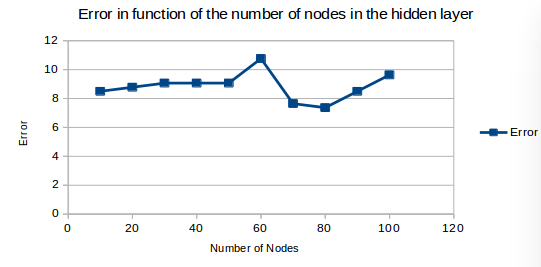
\includegraphics[scale=0.5]{../images/NNPO.png}
   \caption{Class diagram}
  \end{figure}
\subsection{Random forest}
The parameters used for the random forest are the following :
  \begin{itemize}
    \item number of variable randomly selected sqrt(n) (usually the best number);
  \end{itemize}
Results :
\begin{itemize}
  \item Correct classification : 92.07\%;
  \item Wrong classification : 7.93\%;
  \item False positive non ad : 7.082\%;
  \item False positive ad : 0.85\%.
\end{itemize}
\begin{figure}[h]
 \centering
 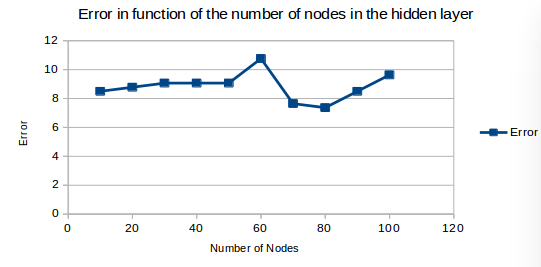
\includegraphics[scale=0.5]{../images/NNPO.png}
 \caption{Class diagram}
\end{figure}
